%Metody statistické indukce. Intervalové odhady. Princip testování hypotéz.

\subsection{Statistická indukce}
Statistická indukce je metoda, která dovoluje stanovit vlastnost celku (\textbf{základního souboru}) na základě pozorování jeho částí (\textbf{náhodného výběru}).
\begin{figure}[H]
\centering
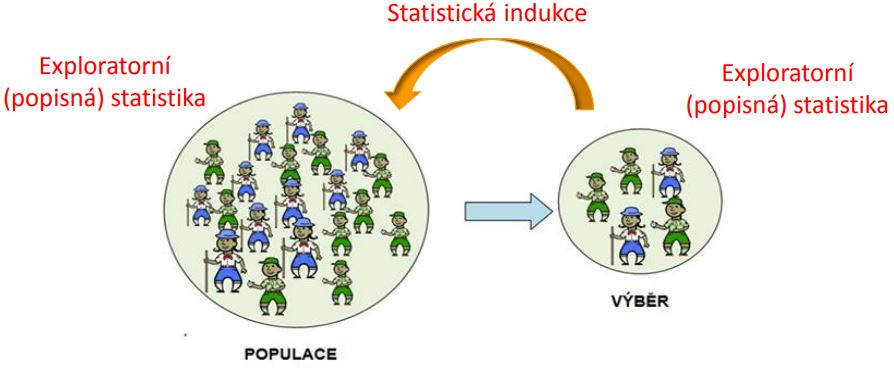
\includegraphics[width=0.6\textwidth]{assets/14_stat_ind}
\end{figure}

\subsubsection{Základní soubor (populace)}
\begin{itemize}
	\item Je množina všech teoreticky možných objektů (např. jedinců) v uvažované situaci = statistický soubor, který je vymezen cílem výzkumu a pro který vyvozujeme závěry výzkumného šetření.
	\item Charakterizuje se \textbf{parametrem}, což je např. výška, váha, IQ, atp.
	\item Má konečný nebo nekonečný (hypotetický) \textbf{rozsah}, který je dán N (např.: N = 150 lidí, opic, rostlin,...).
\end{itemize}
\subsubsection{Výběrový soubor (výběr)}
\begin{itemize}
	\item Je část populace vybrané na základě předem stanovených kritérii resp. pravidel (podmnožina základního souboru).
	\item \textbf{O náhodném výběru} uvažujeme, když splňuje dvě základní vlastnosti:
\begin{itemize}
\item \textbf{pravděpodobnost} zařazení do vzorku je pro všechny statistické jednotky populace \textbf{nenulová},
\item statistické jednotky jsou do vzorku vybrané \textbf{nezávisle} jedna od druhé.
\end{itemize}
	\item \textbf{O reprezentativním výběru} uvažujeme, když výběrový soubor dobře odráží strukturu celého zkoumaného souboru.
\end{itemize}
\subsubsection{Principy statistického usuzování}
\begin{enumerate}
	\item Statistické usuzování znamená zobecňování z výběrových statistik na parametry rozdělení.
	\item Abychom mohli provést statistické usuzování, musíme mít nějakou teorii, jež popisuje náhodné chování sledovaných proměnných.
	\item Existují dva typy výběrových chyb: \textbf{náhodné výběrové chyby} a \textbf{systematické chyby}. Získáním náhodného výběru zmenšujeme systematickou chybu a získáváme podklad pro odhad náhodné výběrové chyby.
	\item Výběrová rozdělení statistik jsou teoretická \textbf{pravděpodobnostní rozdělení}, která popisují vztah mezi výběrovou statistikou a populací.
	\item Směrodatná odchylka výběrového rozdělení statistiky (odhad parametru) se nazývá směrodatná chyba. Odhaduje náhodnou výběrovou chybu vypočítané statistiky (odhadu parametru).
	\item Jak roste velikost výběru, výběrová chyba a směrodatná chyba se zmenšují.
	\item Směrodatná chyba se používá k získání intervalového odhadu parametrů i k testování hypotéz o parametrech rozdělení.
\end{enumerate}
\subsection{Základní metody statistické indukce}
\begin{itemize}
	\item \textbf{Intervalové odhady} (confidence intervals) -- umožnují odhadnout \textbf{nejistotu} v odhadu parametru náhodné veličiny.
	\item \textbf{Testování hypotéz}(hypothesis testing) -- umožnuje posoudit, zda experimentálně získaná data nepopírají předpoklad, který jsem \textbf{před} provedením testování učinili.
\end{itemize}
\begin{figure}[H]
\centering

\includegraphics[width=0.6\textwidth]{assets/14_metody_stat_ind}
\end{figure}
\subsubsection{Intervalové odhady}
\begin{itemize}
\item V praktických aplikacích často určujeme \textbf{odhad příslušného parametru} pomocí intervalového odhadu.
\item Tento odhad je reprezentován intervalem $<t_D, t_H>$, v němž hledaný parametr leží s předem určenou pravděpodobností (spolehlivostí), kterou označujeme $(1 − \alpha)$.
\item neboli parametr populace aproximujeme intervalem, v němž s velkou pravděpodobností příslušný populační parametr leží.
\end{itemize}

\subsubsection{Interval spolehlivosti (konfidenční interval)}
Interval spolehlivosti (konfidenční interval) pro parametr $\theta$ se spolehlivostí $1−\alpha$, kde $\alpha \in <0; 1>$, je \textbf{taková dvojice statistik} $(T_D, T_H)$, že $P(T_D \leq \theta \leq T_H) = 1 − \alpha$.
\begin{figure}[H]
\centering
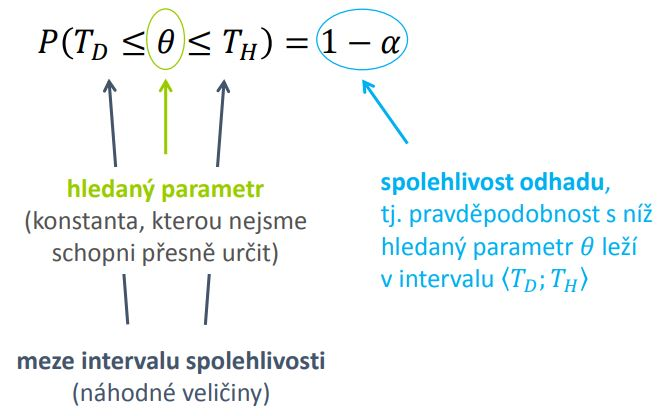
\includegraphics[width=0.6\textwidth]{assets/14_inter_odhad_terminologie}
\end{figure}
\begin{itemize}
	\item \textbf{Intervalový odhad} $t_D,t_H$ je jednou \textbf{z realizací intervalu spolehlivosti}.
	\item Požadavky na interval spolehlivosti:
	\begin{itemize}
		\item Co \textbf{největší spolehlivost} odhadu.
		\item Co \textbf{nejmenší šírka} intervalu spolehlivost. (s rostoucí spolehlivostí se zvětšuje šířka intervalového odhadu a tím \textbf{klesá významnost} takto získané informace. S rostoucím rozsahem výběru se šířka intervalového odhadu snižuje.)
	\end{itemize}
\end{itemize}
\subsubsection*{Typy intervalů spolehlivosti}
	\begin{itemize}
		\item \textbf{oboustranné} 
		\begin{equation*}
				P(\theta < T_D) = P(\theta > T_H) = \frac{\alpha}{2}
		\end{equation*}
		Tyto dvě podmínky zaručují, že $P(T_D \leq \theta \leq T_H) = 1 - \alpha$
		\item \textbf{jednostranné} (odhadujeme--li například délku života nějakého zařízení, je pro nás důležitá pouze dolní mez)
		\begin{itemize}
			\item \textbf{levostranné} $P(\theta \geq T_D^*) = 1 - \alpha$
			\item \textbf{pravostranné} $P(\theta \leq T_H^*) = 1 - \alpha$
		\end{itemize}
	\end{itemize}
\begin{figure}[H]
\centering
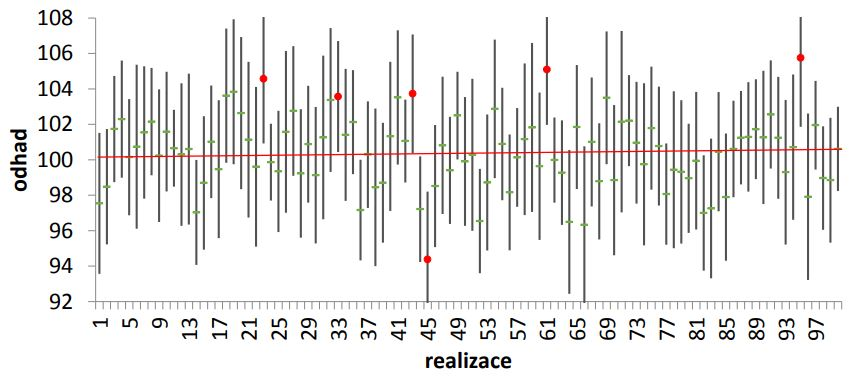
\includegraphics[width=0.6\textwidth]{assets/14_spolehlivost_odhadu}
\end{figure}
\textbf{Co to znamená}, že spolehlivost odhadu je $1- \alpha$? -- Simulace 100 intervalových odhadů  (obrázek výše) střední hodnoty (spolehlivost $0,95$) získaných na základě opakovaných výběrů o rozsahu 30 z populace se střední hodnotou 100. 6 intervalů ze 100 \textbf{neobsahuje skutečnou střední hodnou}.
\subsection{Jak najít intervalový odhad parametru $\theta$?}
\textbf{Obecně:}
\begin{enumerate}
	\item Zvolíme \textbf{vhodnou výběrovou charakteristiku} $T(\mathbf{X})$, jejíž rozdělení známe.
	\item \begin{equation*}
			\begin{split}
				P(x_\frac{\alpha}{2} \leq T(\mathbf{X}) \leq x_{1 - \frac{\alpha}{2}}) &= 1 - \alpha, \\
				P(T(\mathbf{X}) \leq x_{1-\alpha}) &= 1 - \alpha, \\
				P(T(\mathbf{X}) \geq x_\alpha) &= 1 - \alpha.	
			\end{split}
		\end{equation*}
\end{enumerate}

\subsection{Testování hypotéz}
\textbf{Statistická hypotéza} -- předpoklad (tvrzení) o rozdělení náhodné veličiny.
\begin{itemize}
	\item Zdrojem statistických hypotéz jsou například předchozí zkušenosti, teorie, kterou je třeba doložit, požadavky na kvalitu produktu, dohady založené na náhodném pozorování.
	\item \textbf{Příklady} statistických hypotéz:
	\begin{itemize}
		\item Střední životnost žárovek Ed je nižší než výrobcem udávaných 5 let.
		\item Mortalita je u laparoskopických operací nižší než u operací konvenčních.
		\item Průměrné výsledky srovnávacích testů závisí na typu absolvované střední školy.
		\item Pořízený datový soubor je výběrem z populace mající normální rozdělení.
	\end{itemize}
	\item \textbf{Parametrická statistická hypotéza} -- tvrzení ohledně efektu:
	\begin{itemize}
		\item Hypotézy \textbf{o parametru jedné populace} (o střední hodnotě, rozptylu, mediánu, parametru binomického rozdělení,...).
		\item Hypotézy \textbf{o parametrech dvou populací} (srovnávací testy).
		\item Hypotézy \textbf{o parametrech více než dvou populací} (ANOVA, Kruskalův--Wallisův test,...).
	\end{itemize}
	\item \textbf{Neparametrická statistická hypotéza} -- tvrzení o \textbf{jiné vlastnosti} (rozdělení náhodné veličiny) než o jejím parametru (např. hypotézy o typu rozdělení NV, hypotézy o závislosti NV,...)
\end{itemize}
\textbf{Příklad, ověření, zda statistická hypotéza je pravdivá}: Domníváme se, že střední hodnota obsahu cholesterolu v krvu je u české populace 4,7 mmol/l.
	\begin{equation*}
		\begin{split}
			H_0 : \mu = 4.7	 \\
			H_A : \mu \not = 4.7 
		\end{split}
	\end{equation*}
\subsubsection*{Jak tento předpoklad ověřit?}
\begin{itemize}
	\item Zjistíme údaje o obsahu cholesterolu v krvi u 100 náhodně vybraných Čechů.
	\item Průměrný obsah cholesterolu v krvi probandů (tj. jedinců, kteří jsou předmětem zkoumání) byl 5,4 mmol/l.
\end{itemize}
\subsubsection*{Jsou tyto výsledky v souladu s naší hypotézou?}
\begin{itemize}
	\item[$\circ$] I kdyby byla testovaná hypotéza pravdivá, nelze očekávat, že průměrná hodnota pozorovaná ve výběru bude přesně 4,7 mmol/l.
	\item[$\circ$] \textbf{Nulovou hypotézu zamítneme, pokud získané uspořádání výberu bude za předpokladu platnosti nulové hypotézy velmi nepravděpodobné}.
\end{itemize}
Rozhodovací proces, v němž proti sobě stojí nulová a alternativní hypotéza:
\begin{itemize}
	\item \textbf{Nulová hypotéza $\mathbf{H_0}$} -- tvrzení, že efekt je nulový, resp. že neexistuje závislost, že data mají určitý typ rozdělení, ...
	\item \textbf{Alternativní hypotéza $\mathbf{H_A}$ ($\mathbf{H_1}$)} -- tvrzení, popírající hypotézu nulovou (obvykle to, co chceme dokázat).
\end{itemize}

\subsubsection{Klasický přístup při testování hypotéz}
\begin{enumerate}
	\item Formulujeme \textbf{nulovou a alternativní hypotézu}.
	\item Zvolíme tzv. \textbf{testovací statistiku}, tj. výběrovou charakteristiku, jejíž rozdělení závisí na testovaném parametru $\theta$. (Rozdělení testované statistiky za předpokladu platnosti nulové analýzy nazýváme \textbf{nulové rozdělení}.)
	\item Ověříme \textbf{předpoklady testu}! %Hanzi, to musíš zařvat na Edu!
	\item Určíme \textbf{kritický obor} $W^*$, tj. množinu, v níž se, za předpokladu platnosti $H_0$, hodnoty testované statistiky vyskytují s velmi malou pravděpodností.
	\begin{itemize}
		\item Doplňkem k $W^*$ je tzv. \textbf{obor přijetí} $V^*$.
		\item Hranici mezi kritickým oborem a oborem přijetí označujeme jako \textbf{kritická hodnota testu} $t_{krit}$.
	\end{itemize}
	\item Na základě konkrétní realizace výběru určímě \textbf{pozorovanou hodnotu} $X_{OBS}$ testované statistiky. 
	\item Na základě vztahu mezi $X_{OBS}$ a $t_{krit}$ rozhodneme o výsledku testu (\uv{Zamítáme $H_0$.} nebo \uv{Nezamítáme $H_0$.})
\end{enumerate}

\subsubsection{Chyba I. a II. druhu}
\begin{figure}[H]
\centering
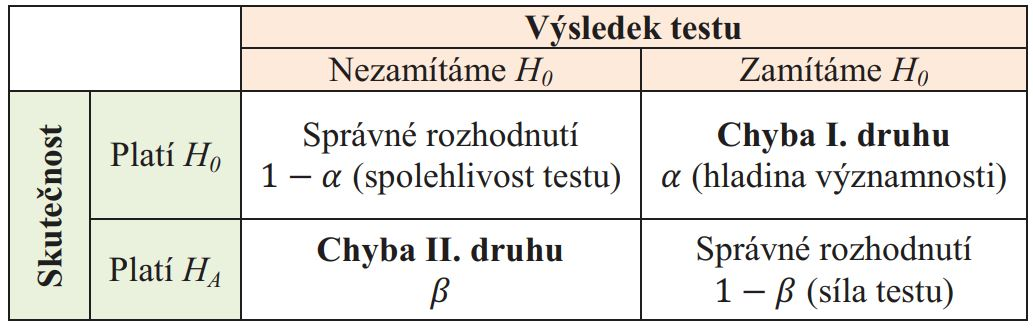
\includegraphics[width=0.6\textwidth]{assets/14_chyba_tab}
\end{figure}
Jestliže nulová hypotéza je ve skutečnosti platná a my ji přesto zamítneme, dopouštíme se chyby, označované jako chyba \textbf{I. druhu}. Pravděpodobnost, že k takovémuto pochybení dojde, nazýváme \textbf{hladina významnosti} a označujeme ji $\alpha$. Platí-li nulová hypotéza a my jsme ji nezamítli, rozhodli jsme správně. Pravděpodobnost tohoto rozhodnutí označujeme $1 − \alpha$ a nazýváme ji \textbf{spolehlivost testu}. Správným rozhodnutím je rovněž \textbf{zamítnutí nulové hypotézy v případě, že je platná hypotéza alternativní}. Tohoto rozhodnutí se dopouštíme s pravděpodobností $1 − \beta$, což bývá označováno jako síla testu. \textbf{Chybou II. druhu} je nezamítnutí nulové hypotézy v případě, že je platná hypotéza alternativní. Pravděpodobnost této chyby označujeme $\beta$.
\begin{figure}[H]
\centering
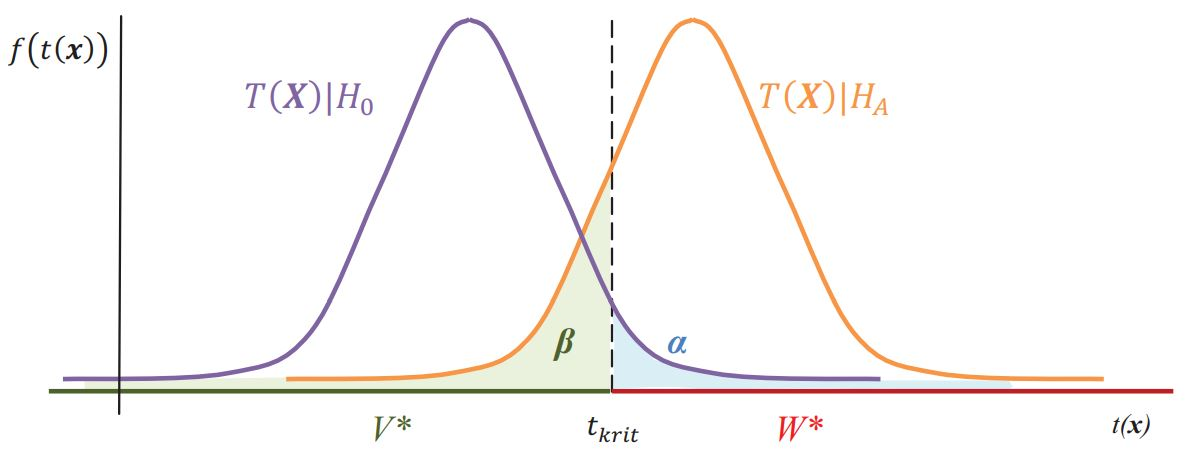
\includegraphics[width=0.6\textwidth]{assets/14_chyba_graf}
\caption{Demonstrace pravděpodobností chyb I. a II. druhu}
\end{figure}
Při testování hypotéz se samozřejmě snažíme postupovat tak, abychom minimalizovali obě chyby, tj. dosáhnout vysoké síly testu (nízkého $\beta$) při co nejnižší hladině významnosti $\alpha$. To však není možné, neboť snížením $\beta$ se zvýší hladina významnosti $\alpha$ a naopak. Proto je třeba najít kompromis mezi požadavky na $\alpha$ a $\beta$.


\subsubsection{Parametrická statistická hypotéza}
\textbf{Jednovýběrové testy}
\begin{itemize}
	\item Test o \textbf{střední hodnotě} (z--test, t--test).
	\item Test o \textbf{rozptylu}.
	\item Test o \textbf{parametru binomického rozdělení}.
	\item Test o \textbf{mediánu} (Wilcoxonův test, Mediánový test).
\end{itemize}
\textbf{Dvouvýběrové testy}
\begin{itemize}
	\item Test o shodě \textbf{dvou středních hodnot} (t--test, Aspinové--Welchův test).
	\item Test o shodě \textbf{rozptylů} (F--test).
	\item Test o shodě \textbf{parametrů dvou binomických rozdělení} (test homogenity dvou binomických rozdělení).
	\item Test o shodě \textbf{mediánů} (Mannův--Whitneyův test).
	\item \textbf{Párové testy} (párový t--test, párový znaménkový test).
\end{itemize}
\textbf{Vícevýběrové testy}
\begin{itemize}
	\item Testy \textbf{shody rozptylů} (Bartletův test, Hartleyův test, Cochranův test, Leveneův test).
	\item \textbf{Analýza rozptylu} (tzv. ANOVA, tj. shody středních hodnot) -- post hoc analýza pro analýzu rozptylu.
	\item Kruskalův--Wallisův test (test \textbf{shody mediánů}) -- post hoc analýza Kruskal--Wallisův test.
\end{itemize}
\textbf{ANOVA}
\begin{itemize}
	\item Test umožnující \textbf{srovnání průměrů více než dvou výběrových souborů}.
	\item Můžeme například zkoumat, zda:
	\begin{itemize}
		\item typ absolvované střední školy ovlivňuje počet bodů dosažených studenty u přijímací zkoušky z matematiky,
		\item použitá medikace ovlivňuje krevní tlak pacientů,
		\item typ použitého hnojiva ovlivňuje výnosy určité plodiny,
		\item pracovní výkon dělníka závisí na umístění stroje, apod.
	\end{itemize}
\end{itemize}